% Welcome! This is the unofficial University of Udine beamer template.

% See README.md for more informations about this template.

% This style has been developed following the "Manuale di Stile"
% (Style Manual) of the University of Udine. You can find the
% manual here: https://www.uniud.it/it/ateneo-uniud/ateneo-uniud/identita-visiva/manuali-immagine-stile/manuale-stile

% Note: for some reason, the RGB values specified in the manual
% do NOT render correctly in Beamer, so they have been redefined
% for this document using the high level chromo-optic deep neural 
% quantistic technology offered by Microsoft Paint's color picker.

% We defined four theme colors: UniBrown, UniBlue, UniGold
% and UniOrange. For example, to write some uniud-brownish
% text, just use: \textcolor{UniBrown}{Hello!}

% Note that [usenames,dvipsnames] is MANDATORY due to compatibility
% issues between tikz and xcolor packages.

\documentclass[usenames,dvipsnames]{beamer}
\usepackage[utf8]{inputenc}
\usepackage{verbatim}
\usepackage[english]{babel}
\usepackage[utf8]{inputenc}
\usepackage{amsmath}
\usepackage{graphicx}
\usepackage[colorinlistoftodos]{todonotes}
\usepackage{xeCJK}
\usepackage{setspace}
\usepackage{amsmath}
\usepackage{multirow}
\usepackage{array}
\usepackage{booktabs}
\usepackage{epsfig}
\usepackage{subfigure}
\usepackage{pythonhighlight}
\usepackage{float}
\usepackage{latexsym}
%\setCJKmainfont{SimSun}
\usepackage{geometry}
\usetheme{uniud}

%%% Bibliography
\usepackage[style=authoryear,backend=biber]{biblatex}
\addbibresource{bibliography.bib}

% Author names in publication list are consistent 
% i.e. name1 surname1, name2 surname2
% See https://tex.stackexchange.com/questions/106914/biblatex-does-not-reverse-the-first-and-last-names-of-the-second-author
\DeclareNameAlias{author}{first-last}

%%% Suppress biblatex annoying warning
\usepackage{silence}
\WarningFilter{biblatex}{Patching footnotes failed}

%%% Some useful commands
% pdf-friendly newline in links
\newcommand{\pdfnewline}{\texorpdfstring{\newline}{ }} 
% Fill the vertical space in a slide (to put text at the bottom)
\newcommand{\framefill}{\vskip0pt plus 1filll}


\title[Tree--Based Models]{An Introduction to Tree--Based Models}
\date[Sept 2018]{Sept 18, 2018}
\author[WISER Club,\,\,Xiamen University]{
  Chunguang Zhang 
  \pdfnewline
}
\institute{WISER Club 2018,\quad Xiamen University}

\begin{document}

\begin{frame}
\titlepage
\end{frame}

\begin{frame}{Outline}
\tableofcontents
\end{frame}
% =============================================================================================================================
% =============================================================================================================================
\section{Decision Tree}
\framepic[0.4]{graphics/thor_iron}{
    \framefill
    \textcolor{white}{\quad \quad \quad Decision Tree}
    \vskip 0.5cm
} 

% =============================================================================================================================
\begin{frame}
\frametitle{决策树—基本流程}
\begin{definition}
决策树=决策树生成(结点分裂递归产生叶结点)+决策树剪枝(防止过拟合)。
\end{definition}

\vskip 0.5cm

\begin{itemize}
  \item \textbf{结点如何分裂}:结点分裂最优属性选择;
  \item \textbf{如何生成叶结点}:生成叶结点条件;
  \item \textbf{剪枝}。
\end{itemize}

\vskip 0.5cm
\end{frame}

% =============================================================================================================================
\begin{frame}
\frametitle{决策树——结点分裂}
结点分裂的目的是为了减小模型的不确定性,不确定性衡量主要基于信息论方法和统计检验方法。
\vskip 0.5cm
\begin{center}
\begin{enumerate}
  \item 信息论\par
    \begin{itemize}
      \item \textbf{信息增益}:样本不充分大时,偏好取值种类多的属性;
      \item \textbf{信息增益率}: 偏好取值不平衡的属性;
      \item \textbf{基尼指数}:样本不充分大时,偏好取值种类多的属性;
      \item TwoValuing
    \end{itemize}
\vskip 0.5cm
  \item 非信息论\par
    \begin{itemize}
      \item \textbf{卡方检验}:QUEST决策树,基于信息论的属性选择有偏;统计检验大法好;
    \end{itemize}
\end{enumerate}
\vskip 0.5cm
\end{center}
\end{frame}
% =============================================================================================================================
\begin{frame}
\frametitle{决策树——结点分裂:信息增益}
假设一节点N包含K类样本,记$p_k$为第k类样本的比例,假定离散属性a有V个不同取值,记$N^v$为N中属性a上取值为$a^v$的样本,记$|S|$为S的样本容量,则:
\begin{itemize}
\item 信息熵计算:
  $$Ent(N) = -\sum_{k=1}^{K}p_klog_2p_k$$ 
\item 信息增益计算:
  $$Gain(N,\,a) = Ent(N)-\sum_{v=1}^{V}\frac{|N^v|}{|N|}Ent(N^v)$$
\end{itemize}
从信息增益准则公式可以看出\textbf{当样本量不充分大}时,若一个划分属性的取值数目越多,则信息增益会越小,因此信息增益偏好属性取值较多的属性进行划分。
\end{frame}
% =============================================================================================================================
\begin{frame}
\frametitle{决策树——结点分裂:信息增益率}
为消除信息增益准则的偏好性,衍生的$C4.5$算法使用信息增益率为基础计算纯度的提升.
\begin{itemize}
  \item 属性分离信息计算:
    $$SplitInformation(N,\, a) = - \sum_{v=1}^{V}\frac{|N^v|}{|N|}log_2\frac{|N^v|}{|N|}$$
  \item 信息增益率计算:
    $$Gain\_ratio(N,\,a) = \frac{Gain(N,\,a)}{SplitInformation(N,\, a)}$$
\end{itemize}
其中SplitInformation(N,\, a)称为分离信息,一般随着属性a取值个数增多而变大。
\end{frame}
% =============================================================================================================================
\begin{frame}
\frametitle{决策树——结点分裂:Gini指数}
\begin{itemize}
  \item Gini信息:
      $$Gini(N^v) = - \sum_{v=1}^{V}\frac{|N^v|}{|N|}(1-\frac{|N^v|}{|N|})$$
  \item Gini指数计算:
      $$Gini\_index(N,\,a) = \sum_{v=1}^{V}\frac{|N^v|}{|N|}Gini(N^v)$$
\end{itemize}
Gini指数本身计算也偏好多值属性,但一般只用在二叉树中。
\end{frame}

% =============================================================================================================================
\begin{frame}
\frametitle{决策树——属性分裂:连续属性}
决策树本质是分类,因此对于连续型属性先进行(伪)离散化处理,通过二分法计算属性最优分割点的信息增益:
\begin{enumerate}
  \item 对特征A进行排序;
  \item 假定特征有V个不同特征值$a^v$,则有V-1个中值$T_A$,计算对每个中值进行分裂的信息增益;
  \item 选择修正信息增益最大的分裂点作为该属性的划分点对数据划分。
\end{enumerate}
    \begin{align*}
            Gain(N,\,A) & = max_{t\in T_A} Gain(N,\,A,\,t)\\
                        & = max_{t\in T_A} (Ent(N) - \sum \frac{|N_t^\lambda|}{|N|}Ent(N_t^\lambda))\\
                    T_A & = \{\frac{a^i+a^{i+1}}{2}|1\le i \le V-1\}\\
      GainRevise(N,\,A) & = Gain(N,\,A) - \frac{log_2(V-1)}{|N|}\\
    \end{align*}
\end{frame}
% =============================================================================================================================
\begin{frame}
\frametitle{决策树——属性分裂:缺失值处理}
决策树在学习过程中对缺失值的处理主要从以下两方面:
        \begin{itemize}
          \item \textbf{有缺失值的属性如何计算分裂指标}\\
            基于每个属性的无缺失样本$\bar{N}$计算信息增益或基尼系数,而后乘以无缺失比例:
            $$Gain(N,\,a) = \rho \times Gain(\bar{N},\,a),\quad \rho = \frac{|\bar{N}|}{|N|}$$
          \item \textbf{有缺失值的样本如何划分}\\
            在基于无缺失的样本属性选择之后,将每个缺失样本按照无缺失样本的后验概率的权重划分入各个子节点中。
        \end{itemize}
\end{frame}

% =============================================================================================================================
\begin{frame}
\frametitle{决策树——属性分裂:多变量}
多变量决策树中采用属性组合进行划分,常用OC1算法:
\begin{itemize}

  \item Coefficients Learning\par
    \begin{itemize}
      \item CART Linear Combination:
        \begin{enumerate}
          \item 基于单变量最优属性$\textbf{x}_{j.}$,建立多变量组合分割平面H:$\sum_{i=1}^{m}a_ix_i+a_{m+1}=0$;
          \item 每次基于当前结点数据优化一个$\sum_{i=1}^{m}a_ix_i-\delta(x_i+\gamma)+a_{m+1}<=0$,寻求最优$a_i,\,a_{m+1}$;
          \item Randomization; 因在步骤(2)中$a_i$都是局部更新,在得到变量组合分割的超平面之后进行扰动优化,生成$(r_1,r_2,\dots, r_{m+1})$加入超平面$H_1 = \sum_{i=1}^{m}(a_i+\alpha r_i)x_i+(a_{m+1}+r_{m+1})$再次优化;
        \end{enumerate}
      \item Recursive Least Square Procedure
        \begin{align*}
          W_k &= W_{k-1}-K_k(X_k^TW_{k-1}-y_k),\quad K_k = P_kK_k\\
          P_k &= P_{k-1} - P_{k-1}X_k[1+X_k^TP_{k-1}X_k]^{-1}X_k^TP_{k-1}
        \end{align*}
    \end{itemize}

  \item Feature Selection:\quad 特征选取类似stepwise。
\end{itemize}
\end{frame}
% =============================================================================================================================
\begin{frame}
\frametitle{决策树——叶结点生成}
\vskip 0.5cm
\begin{itemize}
  \item 当前结点所含样本全部属于同一类别;\vskip 0.36cm


  \item 当前结点属性值为空,没有其他属性进行划分,归类为结点中最多的所属类别;\vskip 0.36cm


  \item 当前结点包含样本为空,样本分布参照父结点的样本分布;\vskip 0.36cm

  \item 预剪枝。
\end{itemize}
\vskip 0.5cm
\end{frame}
% =============================================================================================================================
\begin{frame}
\frametitle{决策树——剪枝}
决策树剪枝目的是为防止过拟合:\vskip 0.36cm
\begin{itemize}
  \item[(1)] 预剪枝\vskip 0.20cm
  在结点分裂前计算泛化指标,无法提升则停止分裂,局部最优化,优点在于模型训练成本降低,但分支未展开可能导致模型欠拟合:
      \begin{itemize}
        \item 设定决策树最大深度;
        \item 节点中的样本个数小于阈值;
        \item 结点分裂的信息增益小于阈值;
      \end{itemize}
\vskip 0.20cm
  \item[(2)] 后剪枝\vskip 0.20cm
  全局最优化,使用目标损失函数正则化来进行剪枝,训练成本高,在生成完整一决策树后从下而上,将非叶结点替换为叶结点计算模型的泛化指标,决定是否转为叶结点。
\end{itemize}
\end{frame}
% =============================================================================================================================
\begin{frame}
\frametitle{决策树——基本算法}
\noindent\rule[0.1\baselineskip]{\textwidth}{0.75pt}\\
\small{
  \textbf{Input:} Train dataset $D = \{(\textbf{x}_i,\,y_i)\,|\,i = 1, 2,\dots, n;\, y_i = 1, 2, ..., k\}$;\\
  \hspace*{28pt} Attributes set $A = \{A_1,A_2,\dots, A_m\}$; Threshold $\epsilon$. \par
  \textbf{Procedure:} TreeGenerate($D,\,A$); Current Node $N$\\
      \hspace*{52pt}  \textbf{if} all instance in $D$ belong to a class j:\\
      \hspace*{68pt}  Label node N as Leaf Node of class j\\
      \hspace*{53pt}  \textbf{elif} $A = \emptyset$ or values of $\textbf{x}_{i}'s$ in $D$ are same:\\
      \hspace*{68pt} Label node N as Leaf Node with the most class
      \hspace*{52pt}  Select a optimal partitioning attributes $A_*$\\
      \hspace*{52pt}  \textbf{if} $Gain(D,\,A_*) < \epsilon$: \textbf{break}\\
      \hspace*{52pt}  \textbf{for} value $a_*^{v}$ in $A_*$:\\
      \hspace*{68pt}  Generate branch for N; denote $D_v$ as subsample\\
      \hspace*{68pt}  \textbf{if} $D_v$ is empty:\\
      \hspace*{84pt}  Label node N as Leaf Node of class j\\
      \hspace*{68pt}  \textbf{else} Denote TreeGenerate($D_v,\, A\backslash{a_*^{v}}$) as child node.
}
\noindent\rule[0.1\baselineskip]{\textwidth}{0.75pt}
\end{frame}
% =============================================================================================================================
\begin{frame}
\frametitle{决策树——基本算法}
不同决策树的算法的区别主要在于:\vskip 0.20cm
\begin{itemize}
  \item 是否二叉树; 
  \item 结点分裂标准;
  \item 连续属性处理;
  \item 是否剪枝方式;
  \item 缺失值处理。
\end{itemize}
\end{frame}
% =============================================================================================================================
\begin{frame}
\frametitle{决策树——算法:ID3}
决策树算法主要分为二叉树与多叉树模型,前者代表有CART和QUEST算法,后者有FACT、C4.5、CHAID、FRIM算法等。
\begin{block}{ID3}
最早的决策树类型,采用信息增益指标进行评估和特征选择,也较为粗糙。
  \begin{enumerate}
    \item 最优属性分割指标:信息增益;
    \item 连续属性处理:无法处理;
    \item 缺失值处理:无法处理;
    \item 剪枝:未进行后剪枝处理;
    \item 适用:数据存于内存中,小规模数据集。
  \end{enumerate}
\end{block}
FIRM算法则是在ID3算法上每个连续性属性划分为10个属性在进行树的生成, 也不进行剪枝。
\end{frame}
% =============================================================================================================================
\begin{frame}
\frametitle{决策树——算法:C4.5}
\begin{block}{C4.5}
  \begin{enumerate}
    \item 最优属性分割指标:\textbf{信息增益结合信息增益率};
    \item 属性处理:二分法处理计算信息增益; 
    \item 缺失值处理:根据后验概率分配到子结点;
    \item 剪枝:采用悲观剪枝法(Pessimistic Error Pruning);
      \begin{itemize}
        \item 内部结点t的样本个数为$N(t)$, 最优子树为$N_t$;
        \item 作为叶结点的错误率$error_t = n(t) +\frac{1}{2}$;
        \item 作为内部结点的错误率 $error_{T_t} = n(T_t)+\frac{N_t}{2}$以及标准差$SE = \sqrt{\frac{n(T_t)(N(t)-n(T_t))}{N(t)}}$
        \item 若$error_{T_t}+SE - error_t>0$,则不分裂;
      \end{itemize} 
    \item 适用:在构造树时需要对数据的属性进行多次扫描和排序,占内存、低效。
  \end{enumerate}
\end{block}
\end{frame}
% =============================================================================================================================
\begin{frame}
\frametitle{决策树——算法:CART}
\begin{block}{CART}
  \begin{enumerate}
    \item 最优属性分割:一般为GINI指数;
    \item 属性处理:二分法处理连续和离散属性,重复性使用;
    \item 缺失值处理:根据后验概率分配到子结点;
    \item 对于树的构建,CART算法会生成尽量大的数目,而后用验证数据集根据损失函数对已生成的树进行剪枝,选择最优子树;
    \item 剪枝:采用独立的验证集剪枝处理,否则剪枝结果为深度最大的子树。
  \end{enumerate}
\end{block}
\end{frame}
% =============================================================================================================================
\begin{frame}
\frametitle{决策树——算法:CART剪枝}
\begin{block}{CART剪枝}
  \begin{itemize}
    \item 计算内部结点t为单结点树(t)和根节点($T_t$)的损失
      $$C_\alpha(t) = C(t)+\alpha,\quad C_\alpha(T_t) = C(T_t)+\alpha|T_t|$$
    \item 当且仅当$C_\alpha(t)<C_\alpha(T_t)$,进行剪枝剪除$T_t$;
    \item 令$g(t) = \frac{C(t)-C(T_t)}{|T_t|-1}$,计算所有内部结点的g(t),依次增加$\alpha$,自下而上在$T_i$中剪除g(t)最小的$T_{t}$得到
    $T_{i+1}$子树;
    \item 利用独立测试集计算独立子树的损失函数,取最优子树。
    \end{itemize}
\end{block}
$C_{\alpha}(T)=\sum_{t=1}^{|T|}N_tH_t + \alpha|T|= \sum_{t=1}^{|T|}N_t(-\sum_k\frac{N_{tk}}{N_t}log\frac{N_{tk}}{N_t})+ \alpha|T|$\\
$\alpha$为树复杂度惩罚系数, $|T|$为结点数目, $N_t$为结点t的样本数,$N_{tk}$为结点t内类k的样本数,$H_t$为结点t的经验熵。
\end{frame}
% =============================================================================================================================
\begin{frame}
\frametitle{决策树——算法:CART回归树}
\begin{block}{CART回归树}
  \textbf{CART回归树}主要先将输入空间划分为M个空间$R_1,R_2,\dots,R_M$,每个空间对应输出值$c_1,c_2,\dots,c_M$,对属性A选择和切分点v时不是选择信息增益或基尼指数,而是最小化:
  $$min_{A,s}[min_{c_1}\sum_{x_i\in \{x|x^A\leq s\}}(y_i-c_1)^2+min_{c_2}\sum_{x_i\in \{x|x^A\geq s\}}(y_i-c_2)^2]$$
  $c_i$在平方误差损失函数下一般取值为$R_i$区间内样本的均值。
\end{block}
\end{frame}
% =============================================================================================================================
\begin{frame}
\frametitle{决策树算法:QUEST}
\begin{itemize}
  \item QUEST会以不同的策略处理特征变量和切分点的选择问题,其算法运行过程要比CART更加快速有效。\vskip 0.36cm

  \item QUEST算法在选择特征变量时,对于定类属性采用卡方检验方法,这点和CHAID类似,对于定矩属性则采用 F 检验方法,选择对应 p 值最小且小于显著性水平的特征变量作为最佳分类变量。
\end{itemize}
\end{frame}
% =============================================================================================================================
\begin{frame}
\frametitle{决策树——Sklearn Decision Tree}
Scikit--learn 模块中使用的决策树算法为CART算法:\par
\vskip 0.5cm
DecisionTreeClassifier(criterion='gini',\, splitter='best',\, \\
\hspace*{32pt}max\_depth=None,\,min\_samples\_split=2,\\
\hspace*{32pt}min\_samples\_leaf=1,\, min\_weight\_fraction\_leaf,\\
\hspace*{32pt}max\_features=None,\, random\_state=None,\\
\hspace*{32pt}max\_leaf\_nodes=None, min\_impurity\_decrease=0.0,\\
\hspace*{32pt}min\_impurity\_split=None,class\_weight=None,\\
\hspace*{32pt}presort=False)
\end{frame} 
% =============================================================================================================================
% =============================================================================================================================

\section{Bagging}
\framepic[0.4]{graphics/widow_witch}{
    \framefill
    \textcolor{white}{\quad \quad \quad \quad Bagging}
    \vskip 0.5cm
}
\framepic[0.20]{graphics/darth}{
  \vfill
    \begin{flushleft}
    \textcolor{gray}{\textbf{\small{Bootstrap\&随机属性选择}}}
    \end{flushleft} 
}

% =============================================================================================================================
% =============================================================================================================================
\section{Boosing}

\framepic[0.4]{graphics/cap_cap}{
    \framefill
    \textcolor{white}{\quad \quad \quad \quad Boosting}
    \vskip 0.5cm
} 

% =============================================================================================================================
\begin{frame}
\frametitle{Boosting——基本流程}
  \begin{figure}
    \centering
    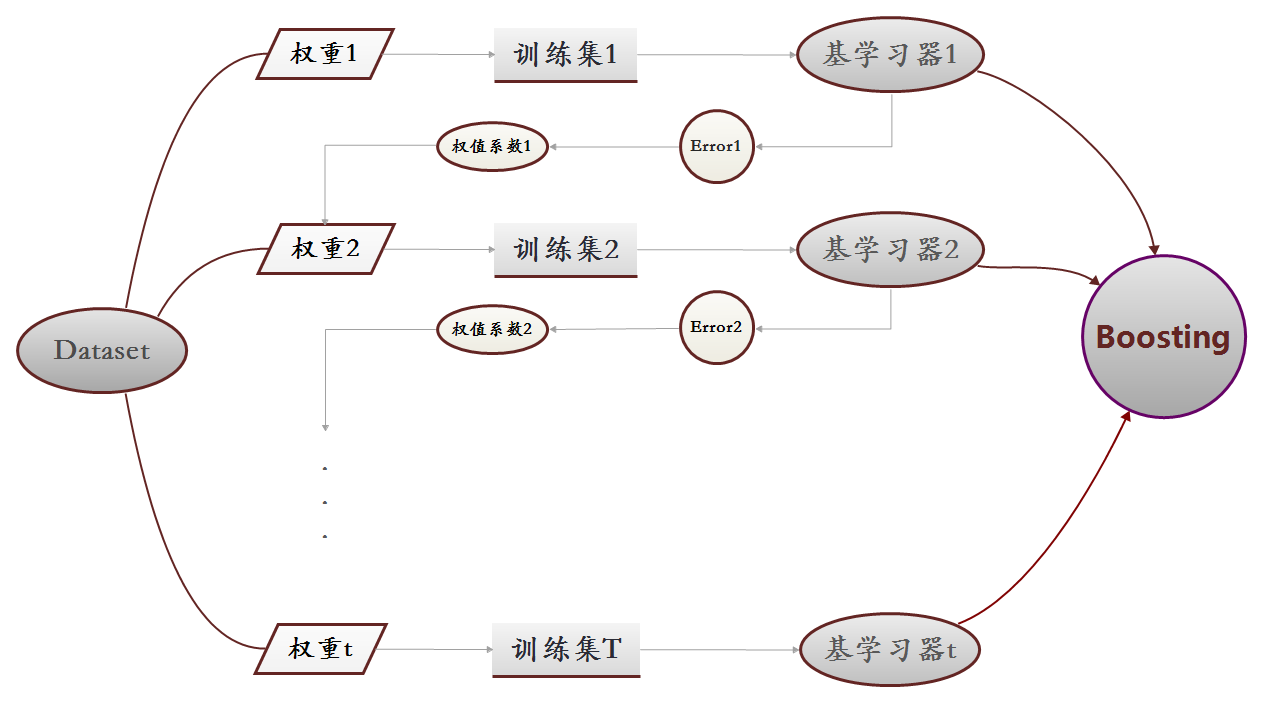
\includegraphics[width=1.02\textwidth]{graphics/Dataset.png}
    \caption{Boosting}
  \end{figure}
\end{frame}
% =============================================================================================================================
\begin{frame}
\frametitle{Boosting——基本流程}
\begin{itemize}
  \item 从初始训练集用初始权重训练出一个基学习器$h_1$;
  \item 根据基学习器的学习误差率$\epsilon$表现更新训练样本权值,使得误差率高的训练样本权值$W_i$增加;
  \item 基于新的样本权值训练基学习器$h_2$;
  \item 迭代进行,直到基学习器数目到达预设数目T,然后根据基学习器的权重$\alpha_i$组合基学习器的训练结果输出。
\end{itemize}
\end{frame}
% =============================================================================================================================
\begin{frame}
\frametitle{Boosting——基本流程}
所以不同的Boosting方法的区别在于以下几点:\vskip 0.36cm
\begin{itemize}
  \item 基学习器误差率的计算即Loss function形式;
  \item 如何根据误差率更新样本权重系数W或计算梯度;
  \item 如何确定基学习器的权重系数。
\end{itemize}
\vskip 0.36cm
针对大部分Boosting算法,基本都是采用加法模型来组合弱分类器,用前向分布算法来改变训练数据的权重和概率分布;
\end{frame}
% =============================================================================================================================
\begin{frame}
\frametitle{Boosting——加法模型}
\begin{itemize}
  \item 考虑K棵树的加法模型:$\hat{y} = \sum_{k=1}^{K}\beta_{k}f(x)$
  \item 解决这一优化问题采用前向分布算法,每次只学习一个基函数及系数,逐步逼近优化目标函数最小化,即
  $$Obj^{t} = \sum_{i=1}^{n}l(y_i, \hat{y}_i^t)+\sum_{i=1}^{t}\Omega(f_i) = \sum_{i=1}^{n}l(y_i, \hat{y}_{i}^{t-1}+f_t(x_i))+\Omega(f_t)+Const.$$
  \item 优化问题转为基于前一学习器预测来最优化当前损失函数,即最小化$\sum_{i=1}^{n}l(y_i, \hat{y}_{i}^{t-1}+f_t(x_i))+\Omega(f_t)$;
  \item 以平方损失函数为例,则模型转为拟合上一轮的残差$$\sum_{i=1}^{n}(y_i-\hat{y}_{i}^{t-1}+f_t(x_i))^2+\Omega(f_t) = \sum_{i=1}^{n}(\epsilon_i - f_i(x))^2 + \Omega(f_t)$$
  \item 损失函数形式及其泰勒展开的不同衍生不同的Boosting。
\end{itemize}
\end{frame}
% =============================================================================================================================
\begin{frame}
\frametitle{AdaBoost}
AdaBoost采用损失函数为最小化指数损失函数$\ell_{exp}(H|W)$的加权加法的\textbf{前向分布算法}模型输出H(x),假定f为真实分布,即
\begin{align*}
  H(\textbf{x}) & = \sum_{t=1}^{T}\alpha_th_t(\textbf{x})\\
    \ell_{exp}(H|W)& = E_{\textbf{x}|W}[exp(-f(x)H(x))]
\end{align*}
AdaBoost作为弱分类器的组合器,基分类器越弱,效果提升越明显,结果也越好,且不容易过拟合,但由于AdaBoost的权值更新方式的原理,AdaBoost对异常数据比较敏感,因异常数据在权值更新中往往会获得较高的权值。
\end{frame}
% =============================================================================================================================
\begin{frame}
\frametitle{AdaBoost for Binary}
\noindent\rule[0.1\baselineskip]{\textwidth}{0.75pt}\\
  \textbf{Algorithm: AdaBoost for Binary Classification}\\
  \noindent\rule[0.1\baselineskip]{\textwidth}{0.5pt}\\
  \textbf{Input:} Train dataset $D = \{(\textbf{x}_i,\,y_i)\,|\,i = 1, 2,\dots, n;\, y_i = -1, 1\}$\\
  \hspace*{32pt} WeakLearn Algorithm I\\
  \hspace*{32pt} Number of Weak Learn Algorithm T\\
  \textbf{Procedure:} 
      \hspace*{1pt} Initializing sample weight vector $W_1(\textbf{x}) = \frac{1}{n}$\par
      \hspace*{58pt} \textbf{for} $t = 1, 2,\dots, T$:\par
          \hspace*{76pt} $h_t = I(D, W_t)$\par
          \hspace*{76pt} $\epsilon_t = P_{\textbf{x}|W_t}(h_t(\textbf{x}) \neq f(\textbf{x}))$\par
          \hspace*{76pt} \textbf{if} $\epsilon_t > 0.5$: \textbf{break}\par
          \hspace*{76pt} $\alpha_t = \frac{1}{2}ln\frac{1-\epsilon_t}{\epsilon_t}$\par
          \hspace*{76pt} $W_{t+1} = \frac{W_t(\textbf{x})}{Z_t}exp[-\alpha f(\textbf{x})h_t(\textbf{x})]$\par
  \textbf{Output:} $H(\textbf{x}) = sign(\sum_{t=1}^{T}\alpha_th_t(\textbf{x}))$\par
  \noindent\rule[0.25\baselineskip]{\textwidth}{0.75pt}\par
\end{frame} 
% =============================================================================================================================
\begin{frame}
\frametitle{AdaBoost for Binary} 
样本权值更新方式: $W_t$
\begin{align*}
  W_{t+1} & = \frac{W_t(\textbf{x})}{Z_t}\times \left \{\begin{array}{ll}
                            exp(-\alpha_t),\, & if\, h_t(\textbf{x})=f(\textbf{x})\\
                              exp(\alpha_t),\, & if\, h_t(\textbf{x})\neq f(\textbf{x})
                            \end{array} \right. \\
        & = \frac{W_t(\textbf{x})}{Z_t}exp(-\alpha f(\textbf{x})h_t(\textbf{x}))
\end{align*}
\end{frame}    
% =============================================================================================================================
% ============================================================================================================================= 
\subsection{AdaBoost}
% =============================================================================================================================
\begin{frame}
\frametitle{AdaBoost for Binary} 
\begin{block}{损失函数解释}
\end{block}
\begin{align*}
    \frac{\partial \ell_{exp}(H|W)}{\partial H(\textbf{x})} 
                    & = -exp(H(\textbf{x}))P(f(\textbf{x})
                      = 1|\textbf{x})+exp(H(\textbf{x}))P(f(\textbf{x})=-1|\textbf{x})\\
      H(\textbf{x}) & = \frac{1}{2}ln\frac{P(f(\textbf{x})=1|\textbf{x})}{P(f(\textbf{x})=-1|\textbf{x})}\\
sign(H(\textbf{x})) & = sign[\frac{1}{2}ln\frac{P(f(\textbf{x})=1|\textbf{x})}{P(f(\textbf{x})=-1|\textbf{x})}]\\
                    & = \left \{\begin{array}{ll}
                              1,\, &$P(f(\textbf{x})=1|\textbf{x}) > P(f(\textbf{x})=-1|\textbf{x})$;\\
                             -1,\, &$P(f(\textbf{x})=1|\textbf{x}) < P(f(\textbf{x})=-1|\textbf{x})$.
                                \end{array} \right.\\
                    & = arg max_{y\in \{-1,1\}} P(f(\textbf{x})=y)
\end{align*}
\end{frame}
% =============================================================================================================================
\begin{frame}
\frametitle{AdaBoost for Binary} 
\begin{block}{权值更新方式:$\alpha_t$}
\end{block}
\begin{align*}
  \ell_{exp}(\alpha_t h_t|W_t) & = E_{x|W_t}[exp(-f(\textbf{x})\alpha_th_t(\textbf{x})] \\
             & = E_{\textbf{x}|W_t}[e^{-\alpha_t}I(f(\textbf{x})=h_t(\textbf{x}))+e^{\alpha_t}I(f(\textbf{x})\neq h_t(\textbf{x}))] \\
             & = e^{-\alpha_t}(1-\epsilon_t) + e^{\alpha_t}\epsilon_t\\
  \frac{\partial \ell_{exp}(\alpha_th_t)}{\partial \alpha_t} & = -e^{-\alpha_t}(1-\epsilon_t) + e^{\alpha_t}\epsilon_t = 0 \\
        \alpha_t & = \frac{1}{2}ln\frac{1-\epsilon_t}{\epsilon_t}
\end{align*}
\end{frame}
% =============================================================================================================================
\begin{frame}
\frametitle{AdaBoost for Binary}
\small{
\begin{align*}
  h_t(\textbf{x})   & = argmin_h \ell_{exp}(H_{t-1}+\alpha_th(\textbf{x})|W) \\
                    & = argmin_h E_{\textbf{x}|W}[exp(-f(\textbf{x}))(H_{t-1}+\alpha_th(\textbf{x}))] \\
                    & = argmin_h E_{\textbf{x}|W}[exp(-f(\textbf{x})H_{t-1})exp(-f(\textbf{x})h(\textbf{x}))]\\
                    & \equiv argmin_h E_{\textbf{x}|W}[exp(-f(\textbf{x})H_{t-1})(1-f(\textbf{x})h(\textbf{x}) + \frac{f^2(\textbf{x})h^2(\textbf{x})}{2})]\\
                    & = argmax_h E_{\textbf{x}|W}[exp(-f(x)H_{t-1})f(x)h(x)] \\
                    & = argmax_h E_{\textbf{x}|W_t}[f(\textbf{x})h(\textbf{x})], \, where\, W_t(\textbf{x}) 
                      = \frac{exp(-f(\textbf{x})H_{t-1})}{E_{\textbf{x}|W}[exp(-f(\textbf{x})H_{t-1}(\textbf{x}))]} \\
                    & = argmax_h E_{\textbf{x}|W_t}[1-2I(f(\textbf{x})\neq h(\textbf{x}))] = argmin_h E_{\textbf{x}|W_t}[I(f(\textbf{x})\neq h(\textbf{x}))]\\
W_{t+1}(\textbf{x}) & = \frac{W_texp(-f(\textbf{x})H_t(\textbf{x}))}{E_{\textbf{x}|W}[exp(-f(\textbf{x})H_t(\textbf{x}))]}
                      = W_texp(-f(\textbf{x})\alpha_th_t)\frac{E_{\textbf{x}|W}[exp(-f(\textbf{x})H_{t-1}(\textbf{x}))]}{E_{\textbf{x}|W}[exp(-f(\textbf{x})H_t(\textbf{x}))]}
\end{align*}
}
\end{frame}
% ============================================================================================================================================  
\begin{frame}
\frametitle{AdaBoost for Multiclass Classification}
AdaBoost 是基于二分类的分类方法,而在多分类中一般有以下几种思路
\begin{itemize}
  \item 只判断是否分类正确与否改变权重;
  \item 判断分类错误为哪一类别,并调整权重;
\end{itemize}
基于以上的思路就产生了AdaBoost.m1和AdaBoost.m2算法。
\end{frame}
% ============================================================================================================================================  
\begin{frame}
\frametitle{AdaBoost.m1 for Multiclass Classification}
AdaBoost.m1 是基于AdaBoost的多分类方法,在更新权值时,分类错误样本权值不更新,而分类正确的样本权重乘以$\frac{\epsilon_t}{1-\epsilon_t}<1$。\par
\noindent\rule[0.1\baselineskip]{\textwidth}{0.75pt}\\
\textbf{Input:} Train dataset $D = \{(\textbf{x}_i,\,y_i)\,|\,i = 1,\dots, n;\, y_i = 1,\dots, k\}$\\
\hspace*{32pt} WeakLearn Algorithm I\\
\hspace*{32pt} Number of Weak Learn Algorithm T\\
\textbf{Procedure:} 
    \hspace*{2pt}Initializing sample weight vector $W_1(\textbf{x}) = \frac{1}{n}$\\
    \hspace*{58pt} \textbf{for} $t = 1, 2,\dots, T$ \textbf{do}\\
        \hspace*{76pt} $h_t = I(D, W_t)$\\
        \hspace*{76pt} $\epsilon_t = P_{\textbf{x}|W_t}(h_t(\textbf{x}) \neq f(\textbf{x}))$\\
        \hspace*{76pt} \textbf{if} $\epsilon_t > 0.5$: \textbf{break}\\
        \hspace*{76pt} $\alpha_t = ln\frac{1-\epsilon_t}{\epsilon_t}$\\
        \hspace*{76pt} $W_{t+1} = \frac{W_t}{Z_t}exp(-\alpha_t(1-[h_t(\textbf{x})\neq y]))$\\
\textbf{Output:} $H(\textbf{x}) = argmax_{y\in C}\sum_{t=1}^{T}\alpha_t[h_t(\textbf{x})=y]$\\
\noindent\rule[0.1\baselineskip]{\textwidth}{0.75pt}\par
\end{frame}
% ============================================================================================================================================  
\begin{frame}
\frametitle{AdaBoost.m2 for Multiclass Classification}
\noindent\rule[0.1\baselineskip]{\textwidth}{0.75pt}\\
\textbf{Input:} Train dataset $D = \{(\textbf{x}_i,\,y_i)\,|\,i = 1, \dots, n;\, y_i = 1,\dots, k\}$;\\
\hspace*{32pt} WeakLearn I; Nums of Iteration T.\\
\textbf{Procedure:} 
    \hspace*{2pt} Initializing sample weight vector $W_1(i) = \frac{1}{n}$;\\
    \hspace*{36pt}$\omega_{i,y}^1 = \frac{W_i}{k-1}$ for $i = 1, 2, \dots, n;\quad y\in \{1,2,\dots,k\}\slash{y_i}$; \\
    \hspace*{32pt} \textbf{for} $t = 1, 2,\dots, T$ \textbf{do}\\
        \hspace*{48pt} $\Omega_i^t = \sum_{y\neq y_i}\omega_{i,y}^t$;\quad $q_t(i,\,y) = \frac{\omega_{i,y}^t}{\Omega_i^t}\,for\,y\neq y_i$;\\
        \hspace*{48pt} $W_t^i = \frac{\Omega_i^t}{\sum_{i=1}^{N}\Omega_i^t}$;\quad $h_t = I(D, W_t)$;\\
        \hspace*{48pt} $\epsilon_t = \frac{1}{2}\sum_{i=1}^{N}W_t(i)(1-h_i(x_i, y_i)+\sum_{i,y\neq y_i}q_t(i,y)h_t(x_i,y))$;\\
        \hspace*{48pt} \textbf{if} $\epsilon_t > 0.5$: \textbf{break}\\
        \hspace*{48pt} $\alpha_t = ln\frac{1-\epsilon_t}{\epsilon_t}$;\\
        \hspace*{48pt} $\omega_{i,y\neq y_i}^{t+1} = \omega_{i,y\neq y_i}^texp(-\frac{1}{2}\alpha_t(1+h_t(x_i,y_i)-h_t(x_i,y)))$;\\
\textbf{Output:} $H(\textbf{x}) = argmax_{y\in C}\sum_{t=1}^{T}\alpha h_t(x,y)$;\\
\noindent\rule[0.1\baselineskip]{\textwidth}{0.75pt}\par
\end{frame}
% ============================================================================================================================================  
\begin{frame}
\frametitle{AdaBoost.m2 for Multiclass Classification}
和AdaBoost.m1原理比较,AdaBoost只关注分类是否错误,而不关注错分在什么样本上,AdaBoost.m2 不仅关注样本分类是否错误,而且关注样本分类错误是在错分在哪一类别上,因此在更新权值时会更新错误分类的权值(如下所示在更新$\epsilon$时更新$\beta$进而提高错误分类样本的权重,同时在最后一步更新$\omega$是降低修改其他类的权重)。
\end{frame}
% ============================================================================================================================================  
\begin{frame}
\frametitle{AdaBoost.R for Regression}
\noindent\rule[0.1\baselineskip]{\textwidth}{0.75pt}\\
\textbf{Input:} Train dataset $D = \{(\textbf{x}_i,\,y_i)\,|\,i = 1, 2,\dots, n;\, y_i \in [0,\,1]\}$;\\
\hspace*{32pt} WeakLearn I; Nums of Iteration T.\\
\textbf{Procedure:} 
    \hspace*{2pt} Initializing sample weight vector $W_1(i) = \frac{1}{n}$;\par
    \hspace*{24pt}$\omega_{i,y}^1 = \frac{W_i*|y-y_i|}{Z}$, where $Z = \sum_{i=1}^{n}W(i)\int_{0}^{1}|y-y_i|dy$; \par
    \hspace*{20pt} \textbf{for} $t = 1, 2,\dots, T$ \textbf{do}\par
        \hspace*{36pt} $W^t = \frac{\omega^t}{\sum_{i=1}^{n}\int_{0}^{1}\omega_{i,y}^t}dy$;\par
        \hspace*{36pt} $h_t = I(D, W_t)$;\par
        \hspace*{36pt} $\epsilon_t = \sum_{1}^{n}|\int_{y_i}^{h_t(x_i)}W_{i,y}^{t}|dy$;\par
        \hspace*{36pt} \textbf{if} $\epsilon_t > 0.5$: \textbf{break}\par
        \hspace*{36pt} $\alpha_t = ln\frac{1-\epsilon_t}{\epsilon_t}$;\\
        \hspace*{36pt} $\omega_{i,y}^{t+1} = \omega_{i,y}^{t}exp(-\alpha[1-I(y\in[y_i, h_t(x_i)] or [h_t(x_i),y_i])]) $;\\
\textbf{Output:} $H(\textbf{x}) = inf \{y:\sum_{t:h_t(y)\leq y}\alpha_t \geq \frac{1}{2}\sum_t \alpha_t\}$;\par
\noindent\rule[0.1\baselineskip]{\textwidth}{0.75pt}
\end{frame}
% ============================================================================================================================================  
\begin{frame}
\frametitle{AdaBoost.R2 for Regression}
\noindent\rule[0.1\baselineskip]{\textwidth}{0.75pt}\\
      \textbf{Input:} Train dataset $D = \{(\textbf{x}_i,\,y_i)\,|\,i = 1,\dots, n;\, y_i \in [0,\,1]\}$;\\
      \hspace*{32pt} WeakLearn I; Nums of Iteration T.\\
      \textbf{Procedure:} 
          \hspace*{2pt} Initializing sample weight vector $W_1(i) = \frac{1}{n}$;\par
          \hspace*{36pt}$\omega_{i,y}^1 = \frac{W_i|y-y_i|}{Z}$, where $Z = \sum_{i=1}^{n}W(i)\int_{0}^{1}|y-y_i|dy$; \par
          \hspace*{32pt} \textbf{for} $t = 1, 2,\dots, T$ \textbf{do}\par
              \hspace*{48pt} $h_t = I(D, W_t)$; $Z^t = max_{i \in \{1,2,\dots,n\}}|y_i-h_t(\textbf{x}_j)|$;\par
              \hspace*{48pt} $e_i^t = \frac{|y_i-h_t(\textbf{x}_j)|}{Z_t}$ for linear loss;\par
              \hspace*{48pt} $\epsilon_t = \sum_{i=1}^{n}e_i^t\omega_i^t$;\par
              \hspace*{48pt} \textbf{if} $\epsilon_t > 0.5$: \textbf{break}\par
              \hspace*{48pt} $\alpha_t = ln\frac{1-\epsilon_t}{\epsilon_t}$;\par
              \hspace*{48pt} $\omega_{i,y}^{t+1} = \frac{\omega_{i,y}^{t}exp(-\alpha_t(1-e_i^t))}{\sum\omega_{i,y}^{t}exp(-\alpha_t(1-e_i^t))}$;\\
      \textbf{Output:} $H(\textbf{x}) = median(\{\alpha_th_t(x),\,i=1,2,...\})$;\par
      \noindent\rule[0.1\baselineskip]{\textwidth}{0.75pt}
\end{frame}
% ============================================================================================================================================  
\begin{frame}
\frametitle{AdaBoost.RT for Regression}
\noindent\rule[0.1\baselineskip]{\textwidth}{0.5pt}\\
\textbf{Input:} Train dataset $D = \{(\textbf{x}_i,\,y_i)\,|\,i = 1, 2,\dots, n;\, y_i \in [0,\,1]\}$;\\
\hspace*{32pt} WeakLearn I; Nums of Iteration T.\\
\hspace*{32pt} threshold $\phi$.\\
\textbf{Procedure:} 
    \hspace*{2pt} Initializing sample weight vector $W_1(i) = \frac{1}{n}$;\par
    %\hspace*{36pt}$\omega_{i,y}^1 = \frac{W_i*|y-y_i|}{Z}$, where $Z = \sum_{i=1}^{n}W(i)\int_{0}^{1}|y-y_i|dy$; \par
    \hspace*{32pt} \textbf{for} $t = 1, 2,\dots, T$ \textbf{do}\par
        \hspace*{48pt} $h_t = I(D, W_t)$;\par
        \hspace*{48pt} $\epsilon_t = \sum_{i=1}^{n}W_t(i)I[|\frac{y_i-h_t(\textbf{x}_j)}{y_i}|>\phi]$\par
        %\hspace*{48pt} \textbf{if} $\epsilon_t > 0.5$ \textbf{then break}\par
        \hspace*{48pt} $\alpha_t = -2ln\epsilon_t$;\par
        \hspace*{48pt} $W_{t+1}(i) = \frac{W_{t}(i)}{Z_t}exp(-\alpha_tI[|\frac{y_i-h_t(\textbf{x}_j)}{y_i}|>\phi])$;\\
\textbf{Output:} $H(\textbf{x}) = \frac{\sum_{i=1}^t\alpha_th_t(x)}{\sum_{i=1}^{t}\alpha_t}$;\par
\noindent\rule[0.1\baselineskip]{\textwidth}{0.75pt}
\end{frame}
% ============================================================================================================================================  
\begin{frame}
\frametitle{AdaBoost——Sklearn}
\begin{block}{Code}
AdaBoostClassifier(base\_estimator,\,n\_estimators,\\
\hspace*{64pt}learning\_rate,\,algorithm)
\end{block}
\begin{block}{Algorithm}
SAMME\&SAMME.R
\end{block}
\end{frame}
% =============================================================================================================================
% ============================================================================================================================= 
\subsection{GB}
% ============================================================================================================================================  
\begin{frame}
\frametitle{Boosting——Boosting Decision Tree}
采用前向分布算法,确定初始提升树之后对第m步的建模为:
\begin{align*}
  f_m(x) & = f_{m-1}(x) + T(x;\Theta_m), \,s.t. \\
    \hat{\Theta}_m &= argmin_{\Theta_m}\sum_{i=1}^{N}L(y_i, f_{m-1}(x_i)+T(x_i;\Theta_m))
\end{align*}
\noindent\rule[0.10\baselineskip]{\textwidth}{0.75pt}\\
  \begin{itemize}
    \item 训练集$T={(x_i,y_i)}$; 初始化$f_0(x) = 0$
    \item for m in 1, 2, ..., M
      \begin{itemize}
        \item 计算残差$r_{mi} = y_i - f_{m-1}(x_i)$
        \item 训练一个回归树 $T(x;\Theta_m)$拟合残差$r_{mi}$
        \item 更新$f_m(x)  = f_{m-1}(x) + T(x;\Theta_m)$
      \end{itemize}
    \item 得到回归树 $f_M(x) = \sum_{m=1}^{M}T(x;\Theta_m)$
  \end{itemize}
\noindent\rule[0.10\baselineskip]{\textwidth}{0.75pt}\par
\end{frame}
% ============================================================================================================================================  
\subsection{GBDT}
\begin{frame}
\frametitle{Boosting——GBDT}
GBDT在基于不同的损失函数上,利用梯度下降法展开目标函数进行优化,进行一阶泰勒展开$f(x+\Delta x) = f(x) + f^{'}(x)\Delta x$,则有
\begin{align*}
  Obj^{(t)} & = \sum_{i=1}^{n}\ell_(y_i, \hat{y}_{i}^{t-1}+f_t(x_i)) \\
        & = \sum_{i=1}^{n}[\ell(y_i, \hat{y}_{i}^{t-1})+\frac{\partial \ell(y_i, \hat{y}_{i}^{t-1})}{\partial \hat{y}_{i}^{t-1}}f_t(x_i)]\\
        & = \sum_{i=1}^{n}[Obj_i^{t-1}+\frac{\partial \ell(y_i, \hat{y}_{i}^{t-1})}{\partial \hat{y}_{i}^{t-1}}f_t(x_i)]
\end{align*}
梯度上升方向为$\frac{\partial l(y_i, \hat{y}_{i}^{t-1})}{\partial \hat{y}_{i}^{t-1}}$,若f取负梯度有$Obj^{(t)} < Obj^{(t-1)}$, 即$f_t = -\epsilon \frac{\partial l(y_i, \hat{y}_{i}^{t-1})}{\partial \hat{y}_{i}^{t-1}},\, \epsilon>0$,$\epsilon$一般就是学习率;\\
\end{frame}
% ============================================================================================================================================  
\begin{frame}
\frametitle{Boosting Decision Tree}
\noindent\rule[0.10\baselineskip]{\textwidth}{0.75pt}
  \begin{itemize}
    \item 训练集$T={(x_i,y_i)}$
    \item 初始化$f_0(x) = 0$
    \item for m in 1, 2, ..., M
      \begin{itemize}
        \item 计算负梯度$r_{mi} = -[\frac{\partial L(y_i, f(x_i))}{\partial f(x_i)}]_{f=f_{m-1}}$
        \item 训练一个回归树 $T(x;\Theta_m)$拟合梯度$r_{mi}$, 得到$T(x;\Theta_m)$的叶结点区域$R_{mj}$
        \item 对$j = 1, 2,\dots, J$, 计算出区域加权输出值使得$c_{mj} = argmin_{c}\sum_{x_i\in R_{mj}}L(f_{m-1}(x_i),\,c)$;
        \item $\alpha_m = argmin_{\alpha}\sum_{i}^{n}L(y_i, f_{m-1}(x_i)+\alpha h_t(x_i))$;
        \item 更新$f_m(x)  = f_{m-1}(x) + \alpha_mh_m(x)$
        %\item 对$j = 1, 2,\dots, J$, 计算出区域加权输出值使得$c_{mj} = argmin_{c}\sum_{x_i\in R_{mj}}L(f_{m-1}(x_i),\,c)$;
        %\item 更新$f_m(x)  = f_{m-1}(x) + \sum_{j=1}^{J}c_{mj}I(x\in R_{mj})$
      \end{itemize}
    \item Return  $f_M(x) = \sum_{m=1}^{M}\alpha_mh_m(x)$
    %\item 得到回归树 $f_M(x) = \sum_{m=1}^{M}\sum_{j=1}^{J}c_{mj}I(x\in R_{mj})$
  \end{itemize}
\noindent\rule[0.10\baselineskip]{\textwidth}{0.75pt}\par
\end{frame}
% ============================================================================================================================================  
\begin{frame}
\frametitle{Boosting Decision Tree}
\begin{itemize}
  \item GBDT的基学习器分裂原则为选择方差增益最高的属性,即:
        $$V_{A_k|D}(d) = \frac{1}{n}(\frac{G_L(A_k)^2}{n_L}+\frac{G_R^2(A_k)}{n_R})$$
  \item GBDT和Boosting Decision Tree的区别在于损失函数取平方误时$c_i$是否直接在基学习器的树中进行优化(平方误的导函数为线性);
\end{itemize}
\end{frame}
% ============================================================================================================================================  
\subsection{XGBoost}
\begin{frame}
\frametitle{XGBoost——正则化}
XGBoost是GBDT的一个拓展,主要对损失函数展开、树模型正则化以及伪并行化进行改进。
\begin{itemize}
  \item 正则化
\end{itemize}
\begin{align*}
          Obj & = \sum_{i}^{n}\ell(y_i, \hat{y}_i^{(t-1)}+f_t(x_i)) + \sum_{t=1}^{T}\Omega(f_t) \\
            & = \sum_{i}^{n}\ell(y_i, \hat{y}_i^{(t-1)}+f_t(x_i)) + \sum_{t=1}^{T}(\gamma |T_t|+\frac{1}{2}\lambda \|\omega\|^2)\\
            & = \sum_{i}^{n}\ell(y_i, \hat{y}_i^{(t-1)}+f_t(x_i)) + \sum_{t=1}^{T}(\gamma |T_t|+\frac{1}{2}\lambda \sum_{m=1}^{M}\omega_{m}^2)
\end{align*}
$|T_t|$为树$T_t$的叶结点个数,$\omega_m(x)=f_t(x)$为m叶结点的取值

\end{frame}
% ============================================================================================================================================  
\begin{frame}
\frametitle{XGBoost——损失函数展开}
\begin{itemize}
  \item 对损失函数利用牛顿法对目标函数进行二阶泰勒展开优化;
\end{itemize}
\begin{align*}
  Obj^{(t)} & = \sum_{i}\ell(y_i, \hat{y}_i^{(t-1)}+f_t(x_i)) + \Omega(f_k) + Constant\\
            & = \sum_{i}[\ell(y_i, \hat{y}_i^{(t-1)}) + \frac{\partial \ell(y_i, \hat{y}_{i}^{t-1})}{\partial \hat{y}_{i}^{t-1}}f_t(x_i) +
                 \frac{1}{2}\frac{\partial^2 l(y_i, \hat{y}_{i}^{t-1})}{\partial (\hat{y}_{i}^{t-1})^2}f_t^2(x_i)] + \Omega(f_k)\\
            & \equiv \sum_{i}[\ell(y_i, \hat{y}_i^{(t-1)}) + g_i\omega_{q(x_i)}+\frac{1}{2}h_i\omega_{q(x_i)^2}]+
                \gamma|T|+\frac{1}{2}\sum_{t=1}^{T}\omega_t^{2}\\
            & = \sum_{t=1}^T[(\sum_{i\in R_t}g_i)\omega_t + \frac{1}{2}(\sum_{i\in R_t}+\lambda)\omega_t^2] + \gamma |T| \\
            & \equiv \sum_{t=1}^T[G_j\omega_t + \frac{1}{2}(H_t+\lambda)\omega_t^2] +\gamma |T|
\end{align*}
\end{frame}

% ============================================================================================================================================  
\begin{frame}
\frametitle{XGBoost——属性分裂}
在对梯度拟合求解最优得到 \\
\quad \quad \quad $\omega_t^{*} = -\frac{G_j}{H_j + \lambda}\quad\Rightarrow\quad 
Obj = -\frac{1}{2}\sum_{T}\frac{G_j^2}{H_j+\lambda}+\gamma |T|$;
\begin{itemize}
  \item GBDT以CART回归树作为基学习器时对属性的最佳分割点的选择衡量标准为最小化均方差,而XGBoost在加入正则化项之后寻找分割点的标准是最大化分裂收益:
\end{itemize}
\begin{align*}
  Obj\_before\_split & = -\frac{1}{2}\frac{(G_L+G_R)^2}{H_L+H_R+\lambda}+\gamma \times 1\\
  Obj\_after\_split & = -\frac{1}{2}[\frac{(G_L)^2}{H_L+\lambda}+\frac{(G_R)^2}{H_R+\lambda}]+\gamma \times 2\\
  node\_split\_gain & = \frac{1}{2}[\frac{(G_L)^2}{H_L+\lambda}+\frac{(G_R)^2}{H_R+\lambda}- \frac{(G_L+G_R)^2}{H_L+H_R+\lambda}]-\gamma
\end{align*}
\end{frame}
% ============================================================================================================================================  
\begin{frame}
\frametitle{XGBoost——贪心分裂}
\noindent\rule[0.10\baselineskip]{\textwidth}{0.75pt}\\
Optimal Splits Search: Greedy Algorithm\\
\noindent\rule[0.10\baselineskip]{\textwidth}{0.5pt}
    \textbf{Input:} Dataset $D=\{(x_i,y_i);\, i = 1,2,\dots, n\};$\par
    \hspace*{32pt} Attribute Set $A = \{A_i;\,i=1,2,\dots,m\}$; Initialize $\lambda$;\par
    \textbf{Procedure:}\par
    \hspace*{32pt} $Gain = 0, G = \sum_{i=1}^{n}g_i,\,H = \sum_{i=1}^{n}h_i$;\par
    \hspace*{32pt} \textbf{for} $i = 1,2,\dots, m$ \textbf{do}\par
    \hspace*{48pt}  $G_L = 0, \, H_L = 0$;\par
    \hspace*{48pt}  \textbf{for} j in sorted(D) \textbf{do}\par
    \hspace*{64pt}  $G_L = G_L+g_j,\, G_R = G - G_L$;\par
    \hspace*{64pt}  $H_L = H_L+h_j,\, H_R = H - H_L$;\par
    \hspace*{48pt}  $score = max\{score, \frac{(G_L)^2}{H_L+\lambda}+\frac{(G_R)^2}{H_R+\lambda}- \frac{(G_L+G_R)^2}{H_L+H_R+\lambda}\};$\par
    \textbf{Output:} Split with max Score\\
\noindent\rule[0.10\baselineskip]{\textwidth}{0.75pt}\par
\end{frame}
% ============================================================================================================================================  
\begin{frame}
\frametitle{XGBoost——分位数估计}
\noindent\rule[0.10\baselineskip]{\textwidth}{0.75pt}\par
Optimal Splits Search: Approximately Algorithm\\
\noindent\rule[0.10\baselineskip]{\textwidth}{0.5pt}
    \textbf{Input:} Dataset $D=\{(x_i,y_i);\, i = 1,2,\dots, n\};$\par
    \hspace*{32pt} Attribute Set $A = \{A_i;\,i=1,2,\dots,m\}$; Initialize $\lambda$;\par
    \textbf{Procedure:}\par
    \hspace*{32pt} \textbf{for} $i = 1,2,\dots, m$ \textbf{do}\par
    \hspace*{48pt}  Propose $S_k = \{s_{k1},s_{k2},\dots,s_{kl}\}$ by percentiles on \\ \hspace*{48pt}feature $A_k$ on per tree or per split;\par
    \hspace*{32pt}  \textbf{for} $i = 1,2,\dots, m$ \textbf{do}\par
    \hspace*{48pt}  $G_{kv} = \sum_{i \in \{i\,|s_{k,v}\geq x_{ik}\geq s_{k,v-1}\}}g_i$\par
    \hspace*{48pt}  $H_{kv} = \sum_{i \in \{i\,|s_{k,v}\geq x_{ik}\geq s_{k,v-1}\}}h_i$\par
    \hspace*{32pt}  Follow the same step in Greedy Algorithm.\par  
    \textbf{Output:} Split with max Score\\
\noindent\rule[0.10\baselineskip]{\textwidth}{0.75pt}\par
\end{frame}
% ============================================================================================================================================  
\begin{frame}
\frametitle{XGBoost——其他特征}
\begin{itemize}
  \item 支持CART(gbtree)树作为基学习器,也支持线性分类器(gblinear);
  \item PreSorted+Exact Split\slash Approximate Percentile Split对所有数据进行预排序后以columb block形式存于内存中,每个变量和标签作为一个Block,之后每次计算分裂时只需要调用即可;
\end{itemize}
\end{frame}
% ============================================================================================================================================  
\subsection{LightGBM}
\begin{frame}
\frametitle{LightGBM}
LightGBM也是GBDT的变种,在算法原理上并未进行改进但有其他特征;
\begin{itemize}
  \item[(1)] 在数据输入模型时,对连续属性进行离散化成k个整数,同时构造宽度为k的直方图存于内存中[bin mapper],后续遍历数据计算分裂时直接使用直方图的累计统计量即可,因此模型时间     运行大幅降低;
  \item[(2)] 与XGBoost采用Level Wise 树生长后进行剪枝的策略不同, LightGBM使用 Leaf Wise 生成策略;
\end{itemize}
\end{frame}
% ============================================================================================================================================  
\begin{frame}
\frametitle{LightGBM}
LightGBM也是GBDT的变种,在算法原理上并未进行改进但有其他特征;
\begin{itemize}
  \item Goss:基于梯度的抽样Boosting;
  \item Exclusive Feature Bundleing:属性集合选择;
  \item Histogram Based Algorithm:直方图算法;
  \item PV Tree FindBestSplit最优属性划分;
  \item DART 算法;
\end{itemize}
\end{frame}
% ============================================================================================================================================  
\begin{frame}
\frametitle{LightGBM——GOSS Sampling}
\noindent\rule[0.10\baselineskip]{\textwidth}{0.75pt}
            \textbf{Input:} Dataset $D=\{(\textbf{x}_i,y_i);\, i = 1,\dots, n\}$; Iterations: T;\par
            \hspace*{12pt} Sampling ratio of large and small gradient: a, b;\par
            \hspace*{12pt} Loss function: $\ell$; Weak Learn: I;\par
            \textbf{Procedure:} Initialize $models = \{\},\,fact = \frac{1-a}{b},\, W = \{1,\dots,1\}$;\par
            \hspace*{28pt} $topN = a\times len(D),\, randN = b\times len(D)$\par
            \hspace*{28pt} \textbf{for} $t=1\, to\, T$ \textbf{do}\par
            \hspace*{44pt}  $h_t(\textbf{x}) = I(\textbf{x}|W_t)$; $\epsilon_t = \ell(y,h_t(\textbf{x})|W_t)$;\par
            \hspace*{44pt}  sorted = SortedIndice(abs($\epsilon_t$));\par
            \hspace*{44pt}  randSet = RandPick(sorted[topN:len(D)],randN)\par

            \hspace*{44pt}  topSet = sorted[1:topN]; usedSet = topSet + randSet;\par
            \hspace*{44pt}  $W_t[randSet]$ *= $fact$; \par
            \hspace*{44pt}  $newModel = \ell(D[usedSet], -\epsilon_t[usedSet],W_t[usedSet])$;\par
            \hspace*{44pt}  models.append(newModel)\par
\noindent\rule[0.10\baselineskip]{\textwidth}{0.75pt}\par
\end{frame}

% ============================================================================================================================================  
\begin{frame}
\frametitle{LightGBM——EFB: Greedy Bundling}
  \noindent\rule[0.10\baselineskip]{\textwidth}{0.75pt}\par
      \textbf{Input:} $F$: features; $K$: max conflict count; $G$: Construct graph\par
      \textbf{Procedure:}\par
      \hspace*{32pt}  $SearchOrder$ = G.sortByDegree();\par
      \hspace*{32pt}  $bundles = \{\}$,\,$bundlesConflict = \{\}$;\par
      \hspace*{48pt}  \textbf{for} $i$ in $searchOrder$ \textbf{do}\par
      \hspace*{64pt}  $needNew$ = True;\par
      \hspace*{64pt}  \textbf{for} $j$ in $len(bundles)$ \textbf{do}\par
      \hspace*{80pt}  $cnt$ = ConflictCnt($bundles[j]$,$F[i]$);\par
      \hspace*{80pt}  \textbf{if} $cnt+bundlesConflict[i]$ $\leq$ K \textbf{then}\par
      \hspace*{96pt}  $bundles[j]$.add($F[i]$);\par
      \hspace*{96pt}  $needNew$ = False;\par
      \hspace*{64pt}  \textbf{if} $needNew$ \textbf{then}\par
      \hspace*{80pt}  Add $F[i]$ as a new bundle to $bundles$;\par
      \textbf{Output:} $bundles$\par
  \noindent\rule[0.10\baselineskip]{\textwidth}{0.75pt}
\end{frame}
% ============================================================================================================================================  
\begin{frame}
\frametitle{LightGBM——EFB: Merge Exclusive Feature}
\noindent\rule[0.10\baselineskip]{\textwidth}{0.75pt}
    \textbf{Input:} $numData$: number of data;\par
    \hspace*{32pt} $F$: One bundle of exclusive features;\par
    \textbf{Procedure:}\par
    \hspace*{32pt} Initialize $binRanges = \{0\}, totalBin = 0$;\par
    \hspace*{32pt} \textbf{for} $f$ in $F$ \textbf{do}\par
    \hspace*{48pt}  $totalBin\, +=\, f.numBin$;\par
    \hspace*{48pt}  $binRanges$.append($totalBin$);\par
    \hspace*{32pt}  newBin = new Bin($numData$);\par
    \hspace*{32pt}  \textbf{for} $i$ = 1 to $F$ \textbf{do}\par
    \hspace*{48pt}  newBin[i]=0\par
    \hspace*{48pt}  \textbf{for} $j$ = 1 to $len(F)$:\par
    \hspace*{64pt}  \textbf{if} $F[j].bin[i]\neq 0$:\par
    \hspace*{80pt}  $newBin[i] = F[j].bin[i]+binRanges[j]$;\par
    \textbf{Output:} $newBins, binRanges$\par
\noindent\rule[0.10\baselineskip]{\textwidth}{0.75pt}\par
\end{frame}
% ============================================================================================================================================  
\begin{frame}
\frametitle{LightGBM——Histogram Based Algorithm}
\noindent\rule[0.10\baselineskip]{\textwidth}{0.5pt}
  \textbf{Input:} Data $D=\{(x_i,y_i);\, i = 1,\dots, n\}$; Tree Max Depth d;\par
  \hspace*{32pt} $NodeSet$: tree nodes, $RowSet$: Data Indices;\par
  \textbf{Procedure:}\par
  \hspace*{32pt} \textbf{for} $i = 1\, to\, d$ \textbf{do}\par
  \hspace*{48pt} \textbf{for} $node$ in $NodeSet$ \textbf{do}\par
  \hspace*{64pt}  usedRows = $RowSet[node]$;\par
  \hspace*{64pt}  \textbf{for} $k = 1\,to\,m$ \textbf{do}\par
  \hspace*{80pt}  H = new Histogram(); Build histogram;\par
  \hspace*{80pt}  \textbf{for} j in usedRows \textbf{do}\par
  \hspace*{96pt}  $bin = D.f[k][j].bin$;\par
  \hspace*{96pt}  $H[bin].y = H[bin].y + D.y[j]$;\par
  \hspace*{96pt}  $H[bin].n = H[bin].n + 1$;\par
  \hspace*{80pt}  Find the best split on histogram H.\par
  \hspace*{48pt}  Update rowSet and NodeSet with best split points.\par 
  \hspace*{48pt}  \dots\par 
\noindent\rule[0.10\baselineskip]{\textwidth}{0.75pt}\par
\end{frame}
% ============================================================================================================================================  
\begin{frame}
\frametitle{LightGBM——PV Tree Find Best Split}
LightGBM基学习器的最佳分裂规则是
\begin{align*}
V_{A_k|D}(d) & = \frac{1}{n}[\frac{(\sum_{x_i \in LargeG_L}g_i + \frac{1-a}{b}\sum_{x_i \in SmallG_L}g_i)^2}{n_L}\\
             &\qquad+\frac{(\sum_{x_i \in LargeG_R}g_i + \frac{1-a}{b}\sum_{x_i \in SmallG_R}g_i)^2}{n_R}]
\end{align*}
传统的分布式计算最佳分裂点是基于Local Worker平行计算之后汇总Global后找出Global BSP再去Local Worker进行分裂;而LightGBM以PV Tree FindBestSplit策略加速寻找最优属性分裂。
\end{frame}
% ============================================================================================================================================  
\begin{frame}
\frametitle{LightGBM——PV: Find Best Split}
\noindent\rule[0.10\baselineskip]{\textwidth}{0.75pt}
  \textbf{Input:} Data $D=\{(x_i,y_i);\, i = 1,\dots, n\}$; Attributes $A = \{A_i;\,i=1,\dots,m\}$;\par
  \textbf{Procedure:}\par
  \hspace*{32pt} \textbf{for all} $A_i$ \textbf{do}\par
  \hspace*{48pt}  Construct Histogram(); H = new Histogram();\par
  \hspace*{48pt}  \textbf{for all} $a$ in $A_i$ \textbf{do}\par
  \hspace*{64pt}  H.binAt(x.bin).Put(x.label);\par
  %\hspace*{48pt}  Find Best Split\par
  \hspace*{48pt}  leftSum = new HistogramSum();\par
  \hspace*{48pt}  \textbf{for all} bin in $H$ \textbf{do}\par
  \hspace*{64pt}  leftSum = leftSum + H.binAt(bin)\par
  \hspace*{64pt}  rightSum = H.AllSum - leftSum\par
  \hspace*{64pt}  split.gain = CalSplitGain(leftSum, rightSum)\par
  \hspace*{64pt}  bestSplit.gain = ChoiceBetterOne(split, bestSplit)\par
  \textbf{Output:} bestSplit\par
\noindent\rule[0.10\baselineskip]{\textwidth}{0.75pt}
\end{frame}
% ============================================================================================================================================  
\begin{frame}
\frametitle{LightGBM——PV Tree}
\noindent\rule[0.10\baselineskip]{\textwidth}{0.75pt}
    \textbf{Procedure:}\par
    \hspace*{32pt}  localHist = ConstructHistogramS(D);\par
    \hspace*{32pt}  \textbf{Local Voting}\par
    \hspace*{32pt}  splits = []\par
    \hspace*{32pt}  \textbf{for} all H in localHist \textbf{do}\par
    \hspace*{48pt}  splits.Push(H.FindBestSplit());\par
    \hspace*{32pt}  localTop = splits.TopKByGain(K);\par
    \hspace*{32pt}  \textbf{Gather all candidates}\par
    \hspace*{32pt}  allCandidates = AllGather(localTop)\par
    \hspace*{32pt}  \textbf{Global Voting}\par
    \hspace*{32pt}  globalTop = all.Candidates.TopKByMajority(2*K);\par
    \hspace*{32pt}  \textbf{Merge Global Histograms}\par
    \hspace*{32pt}  globalHistograms = Gather(globalTop, localHist);\par
    \hspace*{32pt}  bestSplit = globalHistograms.FindBestSplit()\\
\noindent\rule[0.10\baselineskip]{\textwidth}{0.75pt}\par
\end{frame}
% ============================================================================================================================================  
\begin{frame}
\frametitle{LightGBM--DART}
\noindent\rule[0.10\baselineskip]{\textwidth}{0.75pt}
    \textbf{Procedure:}\par
    \hspace*{32pt}  Let N be the total number of trees \par
    \hspace*{32pt}  $S_1 = \{x, -L_x^{'}(0)\}$\par
    \hspace*{32pt}  M = $\{T_i\}$; $T_1$ be a tree trained on the dataset $S_1$\par
    \hspace*{32pt}  \textbf{for} $t = 1\,to\,N$ \textbf{do}\par
    \hspace*{48pt}  D = the subset of M s.t. $T\in M$ is in D with prob $p_{drop}$\par
    \hspace*{48pt}  \textbf{if} D = $\emptyset$ \textbf{then};\par
    \hspace*{64pt}  D = a random element from M\par
    \hspace*{48pt}  $\hat{M}  = M \slash D$; $S_t = \{x, -L_x^{'}(\hat{M}(x))\}$;\par
    \hspace*{48pt}  $T_t$ be a tree trained on the dataset $S_t$;\par
    \hspace*{48pt}  $M = M \cup \{\frac{T_t}{|D|+1}\}$;\par
    \hspace*{48pt}  \textbf{for} $T\in D$ \textbf{do}\par
    \hspace*{64pt}  Multiply T in M by a factor of $\frac{|D|}{|D|+1}$;\par
    \textbf{Output:} M
\noindent\rule[0.10\baselineskip]{\textwidth}{0.75pt}\par
\end{frame}
% ============================================================================================================================================  
\begin{frame}
\frametitle{CatBoost-- Algorithm}
\noindent\rule[0.10\baselineskip]{\textwidth}{0.75pt}
\textbf{Input:} Training Data $D=\{(x_i,y_i);\, i = 1,\dots, n\}$; Iterations T;\\ 
    \hspace*{32pt} Number of Permutations S; Train Mode $M$; $\ell$,$\alpha$;\par
    \hspace*{12pt} $\sigma_i$ = random permutation of $\{1,\dots,n\}$ for $i=1,\dots,s$;\par
    \hspace*{12pt} $S_r(i) = 0,\,r = 1,\dots,s$ for $i=1,\dots,n$;\par
    \hspace*{12pt} $S_{r,j}^{'}(i) = 0,\,r = 1,\dots,s$ for $i=1,\dots,n$, $j = 1, \dots, [log_2n]$;\par
    \hspace*{12pt} \textbf{for} i = 1 to T \textbf{do}\par
    \hspace*{28pt} $grad$ = $ClacGrad(L, S, y)$; $grad^{'}$ = $ClacGrad(L, S^{'}, y);$\par
    \hspace*{28pt} $r = random(1,s)$; $T_t = BuildTree(M, grad_r, grad_r^{'},\sigma_r, \textbf{x})$;\par
    \hspace*{28pt} $leaf_{r,i} = GetLeaf(\textbf{x}_i,T_t, \sigma_r)$ for $r = 0, \dots, s;\,i = 1, \dots, n$;\par
    \hspace*{28pt} \textbf{foreach} $leaf\,R_j^t$ in $T_t$ \textbf{do}\par
    \hspace*{44pt} $b_j^t = -avg(grad_0(i)\,for\,i:leaf_{r,i} = j)$;\par
    \hspace*{28pt} $S, S^{'} = UpdModel(M, leaf, T_t, \{b_j^t\}_j, S, S^{'},grad, grad^{'}, {\sigma_r}_{r=1}^{s})$;\par
\textbf{Output:} $F(x) = \sum_{t=1}^{T}\sum_{j}\alpha b_j^t I(GetLeaf(x, T_t, ApplyMode)==j)$\par
\noindent\rule[0.10\baselineskip]{\textwidth}{0.75pt}
\end{frame}
% ============================================================================================================================================  
\begin{frame}
\frametitle{CatBoost-- BuildTree}
\noindent\rule[0.10\baselineskip]{\textwidth}{0.5pt}
\textbf{Input:} $M, grad_r, grad_r^{'},\sigma_r, \textbf{x}$; T = empty tree;\par
    \hspace*{12pt} \textbf{foreach} step of topdown procedure \textbf{do};\par
    \hspace*{28pt} Form a set $C$ of candidate splits;\par
    \hspace*{28pt} \textbf{for each} $c\in C$ \textbf{do}\par
    \hspace*{44pt} $T_c$ = add split to T; $leaf_i$ = GetLeaf($\textbf{x}_i, T_c, \sigma$);\par
    \hspace*{44pt} \textbf{for each} $leaf\,j\,in\,T_c$ \textbf{do}\par
    \hspace*{60pt} \textbf{for each} $i:\, leaf_i = j$ \textbf{do}\par
    \hspace*{76pt} \textbf{if} M == Plain \textbf{then}\par
    \hspace*{92pt} $\Delta(i) = avg(grad(p):\, leaf_p = j)$ \textbf{else}\par
    \hspace*{92pt} $avg(grad_{[log_2\sigma_r(i)]}^{'}(p):leaf_p = j, \sigma_p<\sigma_i)$;\par
    \hspace*{60pt} $loss(T_c) = \|\Delta-grad\|_2$\par
    \hspace*{44pt} $T = argmin_{T_c}(loss(T_c))$\par
\textbf{Output:} T\\
\noindent\rule[0.10\baselineskip]{\textwidth}{0.5pt}
\end{frame}
% ============================================================================================================================================  
\begin{frame}
\frametitle{CatBoost-- UpdModel}
\noindent\rule[0.10\baselineskip]{\textwidth}{0.75pt}
\textbf{Input:} $Mode, leaf, T_t, \{b_j^t\}_j, S, S^{'},grad, grad^{'}, {\sigma_r}_{r=1}^{s}$\par
    \hspace*{12pt} \textbf{foreach} $leaf\,j\,in\,T$ \textbf{do}\par
    \hspace*{28pt} \textbf{foreach} $i\,s.t.\,leaf_{r,j}=j$ \textbf{do}\par
    \hspace*{44pt} $S_0(i) = S_0(i) + \alpha b_j$;\par
    \hspace*{28pt} \textbf{for} r = 1 to s \textbf{do}\par
    \hspace*{44pt} \textbf{foreach} $i\,s.t.\,leaf_{r,j}=j$ \textbf{do}\par
    \hspace*{60pt} \textbf{if} Mode == Plain \textbf{then}\par
    \hspace*{76pt} $S_r(i) = S_r(i) - \alpha avg(grad_r(p)\, for\, p:\, leaf_{r,p} = j)$;\par
    \hspace*{60pt} \textbf{else:} \textbf{for} l = 1 to $[log_2n]$ \textbf{do}\par
    \hspace*{92pt} $S_{r,l}^{'}(i) = S_{r,l}^{'}(i) - \alpha avg(grad_r(p):\, leaf_{r,p} = j), \sigma_r(p)<2^l$;\par
    \hspace*{76pt} $S_r(i) = S_{r, [log_2\sigma_r(i)]}^{'}(i)$;
\textbf{Output:} $S, S^{'}$\\
\noindent\rule[0.10\baselineskip]{\textwidth}{0.75pt}
\end{frame}
% ============================================================================================================================================  
\begin{frame}
\frametitle{CatBoost-- Categorical Feature}
\begin{itemize}
  \item[(1)] Greedy TBS\par
  TBS 对离散属性数据连续化,处理方法为根据属性取值对应的TARGET取均值:
  $$\hat{x}_i^k = \frac{\sum_{j=1}^n y_iI(x_j^k=x_i^k)}{\sum_{j=1}^n I(x_j^k=x_i^k)}$$
  拉普拉斯平滑处理:
  \begin{align*}
    \hat{x}_i^k & = \frac{\sum_{x_j \in D_k}^n y_iI(x_j^k=x_i^k)+aP}{\sum_{x_j \in D_k}^n I(x_j^k=x_i^k)+a}
  \end{align*}
  \item[(2)] Holdout TBS: Where $D = D_1$
  \item[(3)] Leave one out TBS\par
  \item[(4)] Orderd TBS\par
\end{itemize}
\end{frame}
% % =============================================================================================================================
% % =============================================================================================================================
% \section{Colors}
% \begin{frame}{Colors}
% For this template we defined four colors, following the Style Manual of the University of Udine:
% \begin{itemize}
% \item \textcolor{white}{\marker{\texttt{UniOrange}}}
% \item \textcolor{white}{\marker[UniBlue]{\texttt{UniBlue}}}
% \item \textcolor{white}{\marker[UniBrown]{\texttt{UniBrown}}}
% \item \textcolor{white}{\marker[UniGold]{\texttt{UniGold}}}
% \end{itemize}

% \vskip 0.5cm

% You can use these colors as you want in your presentation. For example, you can \textbf{\textcolor{UniGold}{color the text in gold}} by writing \texttt{\textbackslash\{UniGold\}\{my gold text\}}.

% \vskip 0.5cm

% We also redefined many of the most common \LaTeX{} and Beamer commands, like \texttt{itemize}, \texttt{block}, etc. You will see samples of these commands in the following slides.

% \end{frame}
% % =============================================================================================================================
% % =============================================================================================================================

% \section{Blocks}
% % =============================================================================================================================

% \begin{frame} 
% \frametitle{This is a page with a title and a subtitle} 
% \framesubtitle{And also some blocks.} 
% \begin{block}{Goal of the mission}
% Shoot in the Death Star's exhaust port and destroy it before the it can fire on the Rebel base.
% \end{block} 
% \begin{alertblock}{Take care!}
% TIE Fighters may chase you while approaching the target.
% \end{alertblock} 
% \begin{exampleblock}{Use the force you must}
% Remember your training with Obi-Wan, and use the Force to make the perfect shoot.
% \end{exampleblock} 

% \end{frame}
% % =============================================================================================================================
% % =============================================================================================================================

% \section{Enumerates, itemizes and description}

% \subsection{Enumerates and itemizes}
% % =============================================================================================================================

% \begin{frame}{Enumerates and itemizes}

% This is an example of \texttt{itemize}.
% \begin{itemize}
% 	\item A long time ago in a galaxy far, far away...
% \end{itemize}
% And this is an example of \texttt{enumerate}.

% \begin{enumerate} 
%   \item Go to the Death Star.
%   \item Find the exhaust port.
%   \item Make the perfect shot.
%   \item Become an hero.
% \end{enumerate}
% \end{frame}
% % =============================================================================================================================

% \subsection{Description}

% \begin{frame}[fragile]
% \frametitle{Description}
% This is an example of \texttt{description}.

% \begin{description}
% \item<2->[Vader] \emph{I am} your father.
% \item<1->[Luke] No. No! That's not true! \textbf{That's impossible!}
% \end{description}

% \begin{uncoverenv}<3>
%   \vskip 0.5cm
%   And while we're here, let's have a look to \texttt{verbatim} as well, to see how we made items appear in arbitrary order:
%   \vskip 0.5cm
%   \begin{verbatim}
% \begin{description}
%   \item<2->[This is the first item] one
%   \item<1->[This is the second item] two
% \end{description}
%   \end{verbatim}
% \end{uncoverenv}

% \end{frame}
% % =============================================================================================================================
% % =============================================================================================================================

% \section{Maths}

% \begin{frame}{Maths}
% A formula will look like this: 
% \begin{center}
%  $x^2 + y^2 = z^2$
% \end{center}

% You can number equations as well:
% \begin{equation}
% 1+1=2
% \end{equation}

% \begin{equation}
% 1+1=2 \tag{custom label!}
% \end{equation}

% \vskip 0.5cm

% If you want to use the default \LaTeX{} math fonts, just go to \texttt{beamerfontthemeuniud.sty} and uncomment the line containing `\texttt{\textbackslash usefonttheme[onlymath]\{serif\}}'.

% \end{frame}
% % =============================================================================================================================

% \begin{frame}{Theorems}

% The usual \texttt{theorem}, \texttt{corollary}, \texttt{definition}, \texttt{definitions}, \texttt{fact}, \texttt{example} and \texttt{examples} blocks are available as well.

% \begin{theorem}
% There exists an infinite set.
% \end{theorem}
% \begin{proof}
% This follows from the axiom of infinity.
% \end{proof}
% \begin{example}[Natural Numbers]
% The set of natural numbers is infinite.
% \end{example}

% \end{frame}
% % =============================================================================================================================
% % =============================================================================================================================

% \section{Other blocks}

% \begin{frame}{Other blocks}

% Here we display examples of \texttt{abstract}, \texttt{verse}, \texttt{quotation}, and \texttt{quote}.

% \vskip 0.5cm

% \begin{abstract}
% This is an abstract.
% \end{abstract}
% \begin{verse}
% This is a verse.
% \end{verse}
% \begin{quotation}
% This is a quotation.

% \raggedleft -Han Solo
% \end{quotation}
% \begin{quote}
% A quote this is.

% \raggedleft -Yoda
% \end{quote}

% \end{frame}

% \section{Bibliography and Publications}
% \begin{frame}[fragile]
% \frametitle{Bibliography}

% You can cite an article
% \begin{itemize}
% \item normally using \texttt{\textbackslash cite}, e.g.: (\cite{article1})
% \item or display the full citation using \texttt{\textbackslash fullcite}, e.g.:  \fullcite{article1}
% \end{itemize}

% \vskip 0.5cm
% Look at the code of the following slide to see how to automatically split the bibliography on many slides. You can also use \texttt{\textbackslash nocite\{*\}} to display the non-cited publications as well.

% \end{frame}
% % =============================================================================================================================

% \begin{frame}[t,allowframebreaks]
% \frametitle{Bibliography}

% \nocite{*} % will display the non-cited publications as well. Useful for a publication list.

% \printbibliography

% \end{frame}
% % =============================================================================================================================
% % =============================================================================================================================

% \section{Bonus Commands}

% \begin{frame}[fragile]
% \frametitle{Framecard}

% You can display a frame with a colored background and a huge text in the center using the command \texttt{\textbackslash framecard}.
% \vskip 0.5cm 
% For example, you can write:
% \begin{verbatim}
% \framecard{A SECTION\\TITLE}
% \end{verbatim}

% This will display a frame with a orange background and the phrase "A SECTION TITTLE" in the center. You can also use a custom color with \texttt{\textbackslash framecard}:
% \begin{verbatim}
% \framecard{A SECTION\\TITLE}
% \framecard[UniBlue]{A SECTION TITLE\\
% WITH A CUSTOM COLOR}
% \end{verbatim}
% You can see the results of the commands above in the following slides.

% \end{frame}
% % =============================================================================================================================

% \framecard{A SECTION\\TITLE}
% \framecard[UniBlue]{A SECTION TITLE\\WITH A CUSTOM COLOR}

% \begin{frame}[fragile]
% \frametitle{Framepic}

% You can display a frame with a background image using the command \texttt{\textbackslash framepic}. The image will be \textbf{adapted vertically} to fit the the frame. 

% For example, you can write:
% \begin{verbatim}
% \framepic{graphics/darth}{
% 	\framefill
%     \textcolor{white}{Luke,\\I am your supervisor}
%     \vskip 0.5cm
% }
% \end{verbatim}

% Alternatively, to make the background 50\% transparent, you can write \texttt{\textbackslash framepic[0.5]\{graphics/darth\}...}


% You can see the results of the commands above in the following slides.

% \end{frame}

% % =============================================================================================================================

% \framepic{graphics/darth}{
% 	\framefill
%     \textcolor{white}{Luke,\\I am your supervisor}
%     \vskip 0.5cm
% }
% % =============================================================================================================================

% \framepic[0.5]{graphics/darth}{
% 	\vfill
%     \begin{flushleft}
%     \textcolor{red}{\textbf{Right-aligned text with\\Semi-transparent background}}
%     \end{flushleft}	
% }
% % =============================================================================================================================

% \begin{frame}[t,fragile,allowframebreaks]
% \frametitle{Other bonus commands}

% We provide two other bonus commands:
% \begin{description}
% \item[\texttt{pdfnewline}] you can use \texttt{\textbackslash pdfnewline} to avoid the annoying \texttt{hyperref} related warnings when using newlines in the document's title, author, etc. For example, in this presentation the author is defined as:
% \begin{verbatim}
% \author[Luke Skywalker]{
%   Luke Skywalker, Ph.D.
%   \pdfnewline
%   \texttt{luke.skywalker@uniud.it}
% }
% \end{verbatim}
% \item[\texttt{marker}] you can use \texttt{\textbackslash marker} to highlight some text. The default color is \marker{orange}, but you can also \marker[UniBlue]{use a custom color}. For example:
% \begin{verbatim}
% \marker{Default color}
% \marker[UniBlue]{Custom Color}
% \end{verbatim}
% \item[\texttt{framefill}] you can use \texttt{\textbackslash framefill} to put the text at the bottom of a slide by filling all the vertical space.
% \end{description}

% \end{frame}
% =============================================================================================================================

\end{document}